\item Durante  un año las personas de una ciudad utilizan tres tipos de transportes: metro (M), autobús (A) y coche particular (C). Las probabilidades de que durante el año hayan usado unos u otros transportes son las siguientes: sólo metro = 0,30; sólo autobús = 0,20; sólo coche = 0,15; sólo metro y autobús = 0,10; sólo metro y coche = 0,05; sólo autobús y coche = 0,06; metro,autobús y coche = 0,01.\\
    Calcular las siguientes probabilidades:
    \begin{enumerate}
        \item Que una persona tome al menos dos medios de transporte.\e\\
            $B=$ "la persona toma al menos dos medios de transporte"\\
            $B_{MA}=$ "la persona toma sólo metro y autobús"\\
            $B_{MC}=$ "la persona toma sólo metro y coche"\\
            $B_{AC}=$ "la persona toma sólo autobús y coche"\\
            $B_{T}=$ "la persona toma todos los medios de transporte"\\
            Entonces tenemos que\[P(B)=P(B_{MA}\cup B_{MC}\cup B_{AC}\cup B_{T})\]
            Como los eventos son mutuamente excluyentes\begin{align*}
                P(B)&=P(B_{MA})+P(B_{MC})+P(B_{AC})+P(B_{T})\\
                &=0,10+0,05+0,06+0,01\\
                &=0,22
            \end{align*}
        \item Que una persona viaje en metro y no en autobús.\e\\
            $M=$ "la persona viaja en metro"\\
            $A=$ "la persona viaja en autobús"\\
            Me interesa calcular $P(M-A)=P(M-(M\cap A))=P(M)-P(M\cap A)$ debido a que $M\cap A \subset M$
            \begin{align*}
                P(M)-P(M\cap A)&=[P(\text{sólo en metro})+P(B_{MA})+P(B_{MC})+P(T)]-[P(B_{MA})+P(T)]\\
                &=P(\text{sólo en metro})+P(B_{MC})\\
                &=0,35
            \end{align*}
        \item Que una persona viaje en metro o en coche y no en autobús.\e\\
            $C=$ "la persona viaja en coche"
            \begin{align*}
                P((M\cup C)-A)&=P((M\cup C)-((M\cup C)\cap A))\\
                &=P(M\cup C)-P((M\cup C)\cap A)\\
                &=P(M)+P(C)-P(M\cap C)-P(M\cap A\cup C\cap A)\\
                &=P(M)+P(C)-P(M\cap C)-P(M\cap A)-P(C\cap A)+P(M\cap A\cap C)\\
                &=P(M)+P(C)-[P(B_{MC})+P(T)]-[P(B_{MA})+P(T)]-[P(B_{CA}+P(T))]+P(T)\\
                &=P(M)+P(C)-P(B_{MC})-P(B_{MA})-P(B_{CA})-2P(T)
            \end{align*}
            Tenemos que \begin{align*}
                P(M)=P(\text{sólo en metro})+P(B_{MA})+P(B_{MC})+P(T)=0,3+0,1+0,05+0,01=0,46\\
                P(C)=P(\text{sólo en coche})+P(B_{CA})+P(B_{MC})+P(T)=0,15+0,06+0,05+0,01=0,27
            \end{align*}
            Entonces,\begin{align*}
                P((M\cup C)-A)&=0,46+0,27-0,05-0,1-0,06-2\cdot0,01\\
                &=0,5
            \end{align*}
        \item Que viaje en metro o en autobús y en coche.
            \begin{align*}
                P((M\cup A)\cap C)&=P(M\cap C\cup A\cap C)\\
                &=P(M\cap C)+P(A\cap C)-P(M\cap C\cap A)\\
                &=P(B_{MC})+P(T)+P(B_{AC})+P(T)-P(T)\\
                &=P(B_{MC})+P(B_{AC})+P(T)\\
                &=0,05+0,06+0,01\\
                &=0,12
            \end{align*}
        \item Que una persona vaya a pie.\e\\
            $E=$ "la persona va a pie"\\
            $E^c=$ "la persona toma algún transporte" 
            Se sabe que \[P(E)=1-P(E^c)\]
            En donde \begin{align*}
                P(E^c)&=P(M\cup A\cup C)\\
                &=P(M)+P(A)+P(C)-P(MA)-P(MC)-P(AC)+P(AMC)\\
                &=P(M)+P(A)+P(C)-P(B_{MA})-P(T)-P(B_{MC})-P(T)-P(B_{AC})-P(T)+P(T)\\
                &=P(M)+P(A)+P(C)-P(B_{MA})-P(B_{MC})-P(B_{AC})-2P(T)\\
            \end{align*}
            Se tiene que $P(A)=P(\text{sólo en autobús})+P(B_{MA})+P(B_{CA})+P(T)=0,37$. Entonces,
            \[P(E^c)=0,46+0,37+0,27-0,1-0,05-0,06-2\cdot0,01=0,87\]
            Por lo tanto \[P(E)=1-0,87=0,13\]
            También se podría haber hecho un diagrama de Venn y analizar cada situación como sigue
            \begin{enumerate}
                \item La persona toma al menos dos medios de transporte\e\\
                    Si toma al menos dos, el sector de interés es
                    \begin{center}
                        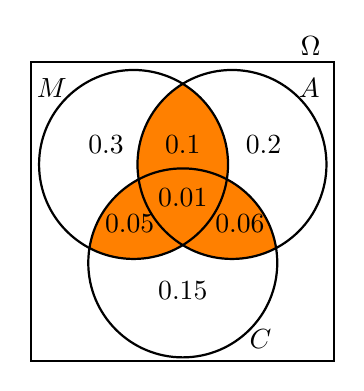
\begin{tikzpicture}
                            [thick,
                            set/.style = {circle,
                                        minimum size = 2cm}]
                            \fill[white] (-1.3,-2.5) rectangle (2.55,1.3);
                            \begin{scope}
                                \clip (1.25,0) circle (1.2);
                                \clip (0,0) circle (1.2);
                                \fill[orange] (-1.3,-2.5) rectangle (2.55,1.3);
                            \end{scope}
                            \begin{scope}
                                \clip (1.25,0) circle (1.2);
                                \clip (0.625,-1.25) circle (1.2);
                                \fill[orange] (-1.3,-2.5) rectangle (2.55,1.3);
                            \end{scope}
                            \begin{scope}
                                \clip (0,0) circle (1.2);
                                \clip (0.625,-1.25) circle (1.2);
                                \fill[orange] (-1.3,-2.5) rectangle (2.55,1.3);
                            \end{scope}
                            \draw [draw=black] (-1.3,-2.5) rectangle (2.55,1.3);
                            % Conjunto Metro
                            \node[set,label={135:$M$}] (M) at (0,0) {};
                            % Conjunto autobús
                            \node[set,label={45:$A$}] (A) at (1.25,0) {};
                            % Conjunto coche
                            \node[set,label={315:$C$}] (C) at (0.625,-1.25) {};
                            % Dibujo conjuntos
                            \draw (0,0) circle(1.2cm);
                            \draw (1.25,0) circle(1.2cm);
                            \draw (0.625,-1.25) circle(1.2cm);
                            % Set intersection label
                            \node at (-0.35,0.25) {0.3};
                            \node at (1.65,0.25) {0.2};
                            \node at (0.625,0.25) {0.1};
                            \node at (0.625,-1.6) {0.15};
                            \node at (barycentric cs:A=1,M=1,C=1) {0.01};
                            \node at (-0.05,-0.75) {0.05};
                            \node at (1.35,-0.75) {0.06};
                            \node at (2.25,1.5) {$\Omega$};
                        \end{tikzpicture}
                    \end{center}
                    Con lo cual\[P(\text{al menos dos transportes})=0,1+0,01+0,05+0,06=0,22\]
                \item Viaje en metro y no en autobús
                    \begin{center}
                        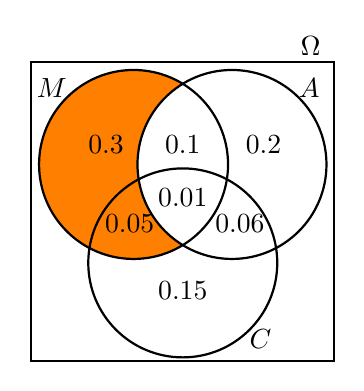
\begin{tikzpicture}
                            [thick,
                            set/.style = {circle,
                                        minimum size = 2cm}]
                            \fill[orange] (0,0) circle (1.2);
                            \begin{scope}
                                \clip (1.25,0) circle (1.2);
                                \clip (0,0) circle (1.2);
                                \fill[white] (0,0) circle (1.2);
                            \end{scope}
                            \draw [draw=black] (-1.3,-2.5) rectangle (2.55,1.3);
                            % Conjunto Metro
                            \node[set,label={135:$M$}] (M) at (0,0) {};
                            % Conjunto autobús
                            \node[set,label={45:$A$}] (A) at (1.25,0) {};
                            % Conjunto coche
                            \node[set,label={315:$C$}] (C) at (0.625,-1.25) {};
                            % Dibujo conjuntos
                            \draw (0,0) circle(1.2cm);
                            \draw (1.25,0) circle(1.2cm);
                            \draw (0.625,-1.25) circle(1.2cm);
                            % Set intersection label
                            \node at (-0.35,0.25) {0.3};
                            \node at (1.65,0.25) {0.2};
                            \node at (0.625,0.25) {0.1};
                            \node at (0.625,-1.6) {0.15};
                            \node at (barycentric cs:A=1,M=1,C=1) {0.01};
                            \node at (-0.05,-0.75) {0.05};
                            \node at (1.35,-0.75) {0.06};
                            \node at (2.25,1.5) {$\Omega$};
                        \end{tikzpicture}
                    \end{center}
                    De donde se sigue que\[P(\text{metro y no autobús})=0,3+0,05=0,35\]
                \item Metro o coche y no autobús
                    \begin{center}
                        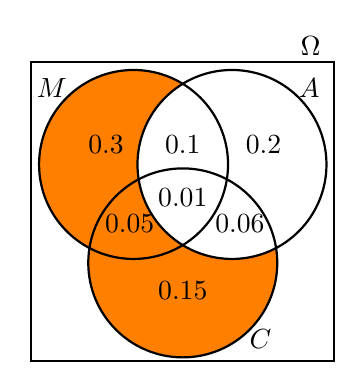
\begin{tikzpicture}
                            [thick,
                            set/.style = {circle,
                                        minimum size = 2cm}]
                            \fill[orange] (0,0) circle (1.2);
                            \begin{scope}
                                \clip (1.25,0) circle (1.2);
                                \clip (0,0) circle (1.2);
                                \fill[white] (0,0) circle (1.2);
                            \end{scope}
                            \fill[orange] (0.625,-1.25) circle (1.2);
                            \begin{scope}
                                \clip (1.25,0) circle (1.2);
                                \clip (0.625,-1.25) circle (1.2);
                                \fill[white] (1.25,0) circle (1.2);
                            \end{scope}
                            \draw [draw=black] (-1.3,-2.5) rectangle (2.55,1.3);
                            % Conjunto Metro
                            \node[set,label={135:$M$}] (M) at (0,0) {};
                            % Conjunto autobús
                            \node[set,label={45:$A$}] (A) at (1.25,0) {};
                            % Conjunto coche
                            \node[set,label={315:$C$}] (C) at (0.625,-1.25) {};
                            % Dibujo conjuntos
                            \draw (0,0) circle(1.2cm);
                            \draw (1.25,0) circle(1.2cm);
                            \draw (0.625,-1.25) circle(1.2cm);
                            % Set intersection label
                            \node at (-0.35,0.25) {0.3};
                            \node at (1.65,0.25) {0.2};
                            \node at (0.625,0.25) {0.1};
                            \node at (0.625,-1.6) {0.15};
                            \node at (barycentric cs:A=1,M=1,C=1) {0.01};
                            \node at (-0.05,-0.75) {0.05};
                            \node at (1.35,-0.75) {0.06};
                            \node at (2.25,1.5) {$\Omega$};
                        \end{tikzpicture}
                    \end{center}
                    Por ende\[P(\text{metro o coche y no autobús})=0,3+0,05+0,15=0,5\]
                \item Metro o autobús y coche.
                    \begin{center}
                        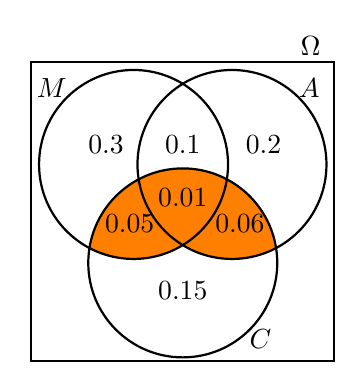
\begin{tikzpicture}
                            [thick,
                            set/.style = {circle,
                                        minimum size = 2cm}]
                            \fill[white] (0.625,-1.25) circle (1.2);
                            \begin{scope}
                                \clip (1.25,0) circle (1.2);
                                \clip (0.625,-1.25) circle (1.2);
                                \fill[orange] (1.25,0) circle (1.2);
                            \end{scope}
                            \begin{scope}
                                \clip (0,0) circle (1.2);
                                \clip (0.625,-1.25) circle (1.2);
                                \fill[orange] (0.625,-1.25) circle (1.2);
                            \end{scope}
                            \draw [draw=black] (-1.3,-2.5) rectangle (2.55,1.3);
                            % Conjunto Metro
                            \node[set,label={135:$M$}] (M) at (0,0) {};
                            % Conjunto autobús
                            \node[set,label={45:$A$}] (A) at (1.25,0) {};
                            % Conjunto coche
                            \node[set,label={315:$C$}] (C) at (0.625,-1.25) {};
                            % Dibujo conjuntos
                            \draw (0,0) circle(1.2cm);
                            \draw (1.25,0) circle(1.2cm);
                            \draw (0.625,-1.25) circle(1.2cm);
                            % Set intersection label
                            \node at (-0.35,0.25) {0.3};
                            \node at (1.65,0.25) {0.2};
                            \node at (0.625,0.25) {0.1};
                            \node at (0.625,-1.6) {0.15};
                            \node at (barycentric cs:A=1,M=1,C=1) {0.01};
                            \node at (-0.05,-0.75) {0.05};
                            \node at (1.35,-0.75) {0.06};
                            \node at (2.25,1.5) {$\Omega$};
                        \end{tikzpicture}
                    \end{center}
                    \[P(\text{metro o autobús y coche})=0,05+0,01+0,06=0,12\]
                \item Que vaya a pie.
                \begin{center}
                    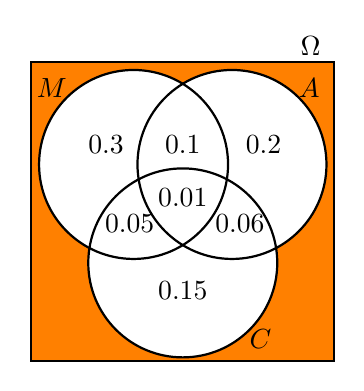
\begin{tikzpicture}
                        [thick,
                        set/.style = {circle,
                                    minimum size = 2cm}]
                        \fill[orange] (-1.3,-2.5) rectangle (2.55,1.3);
                        \begin{scope}
                            \clip (1.25,0) circle (1.2);
                            \fill[white] (1.25,0) circle (1.2);
                        \end{scope}
                        \begin{scope}
                            \clip (0.625,-1.25) circle (1.2);
                            \fill[white] (0.625,-1.25) circle (1.2);
                        \end{scope}
                        \begin{scope}
                            \clip (0,0) circle (1.2);
                            \fill[white] (0,0) circle (1.2);
                        \end{scope}
                        \draw [draw=black] (-1.3,-2.5) rectangle (2.55,1.3);
                        % Conjunto Metro
                        \node[set,label={135:$M$}] (M) at (0,0) {};
                        % Conjunto autobús
                        \node[set,label={45:$A$}] (A) at (1.25,0) {};
                        % Conjunto coche
                        \node[set,label={315:$C$}] (C) at (0.625,-1.25) {};
                        % Dibujo conjuntos
                        \draw (0,0) circle(1.2cm);
                        \draw (1.25,0) circle(1.2cm);
                        \draw (0.625,-1.25) circle(1.2cm);
                        % Set intersection label
                        \node at (-0.35,0.25) {0.3};
                        \node at (1.65,0.25) {0.2};
                        \node at (0.625,0.25) {0.1};
                        \node at (0.625,-1.6) {0.15};
                        \node at (barycentric cs:A=1,M=1,C=1) {0.01};
                        \node at (-0.05,-0.75) {0.05};
                        \node at (1.35,-0.75) {0.06};
                        \node at (2.25,1.5) {$\Omega$};
                    \end{tikzpicture}
                \end{center}
                \[P(\text{vaya a pie})=1-(0,3+0,1+0,2+0,05+0,01+0,06+0,15)=0,13\]
            \end{enumerate}
    \end{enumerate}